\documentclass[12pt]{article}

% Paketi za podršku jeziku, matematici i slikama
\usepackage[utf8]{inputenc}
\usepackage[T1]{fontenc}
\usepackage[serbian]{babel}
\usepackage{amsmath}
\usepackage{graphicx}
\usepackage{hyperref}
\usepackage{geometry}
\geometry{a4paper, margin=1in}

% Naslov dokumenta
\title{Predviđanje koncentracije PM2.5 čestica primjenom modernih modela vremenskih serija i dekompozicije trenda}
\author{}
\date{}

\begin{document}
	
	\maketitle
	
	\section{Opis problema}
	Kvalitet vazduha u urbanim sredinama direktno zavisi od složene interakcije između antropogenih faktora i meteoroloških prilika. Problem koji ovaj projekat rješava je predviđanje budućih vrijednosti PM2.5 čestica na osnovu istorijskih podataka, uz jasno razgraničenje varijacija u podacima.
	
	Ključni pojam analize:
	\begin{itemize}
		\item \textbf{Sezonalnost:} Pravilni, periodični obrasci fiksne dužine. U ovom istraživanju fokus je na \textit{godišnjoj sezonalnosti} (razlika između grejne sezone i ljetnjeg perioda) i \textit{dnevnoj sezonalnosti} (varijacije u zavisnosti od jutarnjih i popodnevnih saobraćajnih špiceva).
	\end{itemize}
	
	\begin{figure}[h]
		\centering
		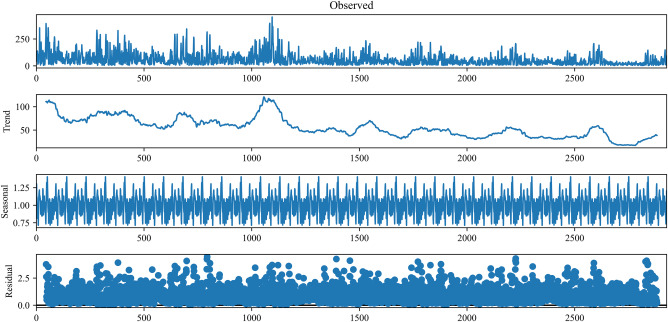
\includegraphics[width=0.8\textwidth]{primjer1.jpg} 
		\caption{Primjer dekompozicije vremenske serije (Trend, Sezonalnost, Reziduali)}
	\end{figure}
	
	\section{Skup podataka (Dataset)}
	\textbf{Izvor:} UCI Machine Learning Repository - Beijing Multi-Site Air-Quality.
	
	\textbf{Opis skupa:} Skup obuhvata satna mjerenja zagađenja u periodu od \textbf{1. marta 2013. do 28. februara 2017. godine}. Ukupan broj mjerenja po svakoj od 12 mernih stanica iznosi \textbf{35,064 uzoraka}. Analiza će biti fokusirana na stanicu \textit{Aotizhongxin}, koja sadrži podatke o PM2.5 koncentraciji, temperaturi, pritisku, vlažnosti vazduha i smjeru vjetra.
	
	\subsection*{Istraživačka pitanja}
	Tokom eksplorativne analize podataka (EDA), projekat će odgovoriti na sljedeća pitanja:
	\begin{enumerate}
		\item Koji meteorološki faktor (brzina vjetra, temperatura ili vlažnost) ima najjaču korelaciju sa skokovima zagađenja?
		\item Postoji li jasan obrazac zagađenja u zavisnosti od doba dana ili u zavisnosti od doba godine?
	\end{enumerate}
	
	\section{Metodologija}
	
	\subsection*{I Faza: Pretprocesiranje podataka}
	Podaci sadrže NaN vrijednosti koje nastaju usljed kvarova na senzorima. Primijeniće se linearna interpolacija za popunjavanje kratkih prekida, dok će se za duže periode koristiti sezonska zamjena srednjom vrijednošću.
	
	\subsection*{II Faza: Eksplorativna analiza i statistički testovi}
	Razlaganje serije na sezonalnost vršiće se pomoću \texttt{STL} dekompozicije. Stacionarnost će biti testirana Augmented Dickey-Fuller (ADF) testom.
	
	\subsection*{III Faza: Modelovanje (Poređenje modela)}
	Umjesto samo klasičnih metoda, implementiraće se i uporediti:
	\begin{itemize}
		\item \textbf{ARIMA (klasični model):} Kao osnovni statistički benchmark model.
		\item \textbf{Prophet (Meta):} Savremeni model otporan na nedostajuće vrijednosti i osjetljiv na praznike i višestruku sezonalnost (dnevnu i godišnju).
		\item \textbf{LSTM (Long Short-Term Memory):} Arhitektura dubokog učenja (RNN) specijalizovana za hvatanje nelinearnih zavisnosti u vremenskim serijama.
	\end{itemize}
	
	\section{Svrha i cilj predikcije}
	Cilj projekta je \textbf{kratkoročna prognoza (short-term forecasting)} koncentracije PM2.5 čestica za narednih **24 sata**. Ovakav model ima praktičnu primjenu u sistemima ranog upozoravanja građana na opasne uslove kvaliteta vazduha.
	
	\section{Način evaluacije}
	Evaluacija će se vršiti na testnom skupu (posljednjih 6 mjeseci podataka). Koristiće se \textbf{RMSE} i \textbf{MAE} metrike. 
	\[ RMSE = \sqrt{\frac{1}{n}\sum_{i=1}^{n}(y_i - \hat{y}_i)^2} \]
	
	\section{Tehnologije}
	\begin{itemize}
		\item \textbf{Programski jezik:} Python 3.x.
		\item \textbf{Biblioteke:} \texttt{Pandas}, \texttt{Statsmodels}, \texttt{Prophet}, \texttt{TensorFlow/Keras} (za LSTM).
	\end{itemize}
	
	\section{Literatura}
	\begin{itemize}
		\item Kaggle - Beijing Air Quality Analysis \href{https://www.kaggle.com/datasets/sid321axn/beijing-multisite-airquality-data-set}{[Link]}.
		\item Air Quality Prediction using Machine Learning \href{https://github.com/topics/air-quality-prediction}{[Link]}.
		\item Istraživački rad (ScienceDirect): \textit{Forecasting of Beijing PM2.5 with a hybrid ARIMA model...}.
	\end{itemize}
	
	
\end{document}